\begin{figure}[H]
    \centering
    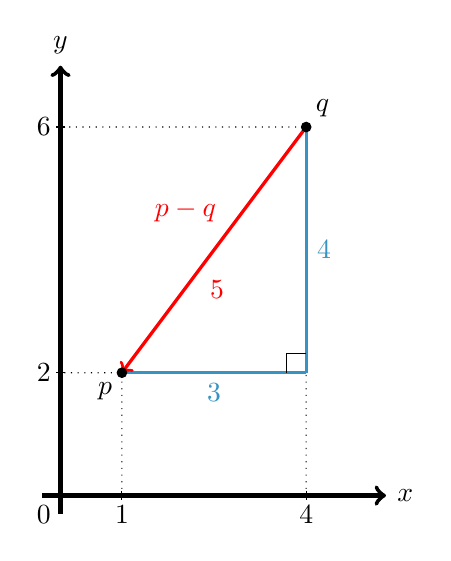
\begin{tikzpicture}[scale=0.78]
        \coordinate (p) at (1,2);
        \coordinate (q) at (4,6);
        \coordinate (a) at (4,2);

        % Eixos coordenados.
        \draw[->, ultra thick] (-0.3,0) -- (5.3,0) node[right] {$x$};
        \draw[->, ultra thick] (0,-0.3) -- (0,7.0) node[above] {$y$};
        \node[below left] at (0,0) {$0$};

        % Marcas principais nos eixos.
        \foreach \x in {1,4} {
            \draw (\x,0.08) -- (\x,-0.08);
            \node[below] at (\x,0) {$\x$};
        }
        \foreach \y in {2,6} {
            \draw (0.08,\y) -- (-0.08,\y);
            \node[left] at (0,\y) {$\y$};
        }

        % Projecoes dos pontos sobre os eixos.
        \draw[dotted] (1,0) -- (p) -- (0,2);
        \draw[dotted] (4,0) -- (q) -- (0,6);

        % Triangulo retangulo associado ao deslocamento.
        \draw[Cerulean!80!black, very thick] (p) -- (a)
            node[midway, below] {$3$};
        \draw[Cerulean!80!black, very thick] (a) -- (q)
            node[midway, right] {$4$};
        \draw (a) ++(-0.32,0) -- ++(0,0.32) -- ++(0.32,0);

        % Segmento orientado de q ate p.
        \draw[Red, very thick, ->] (q) -- (p)
            node[pos=0.43, above left] {$p-q$}
            node[pos=0.58, below right] {$5$};

        % Pontos.
        \filldraw[black] (p) circle (2.2pt) node[below left] {$p$};
        \filldraw[black] (q) circle (2.2pt) node[above right] {$q$};
    \end{tikzpicture}
    \caption{Distância entre $p=(1,2)$ e $q=(4,6)$ em $\mathbb R^2$.}
    \label{fig:distanciaRn}
\end{figure}
